\documentclass{standalone}
\usepackage{tikz}
\usetikzlibrary{patterns, positioning}

\begin{document}
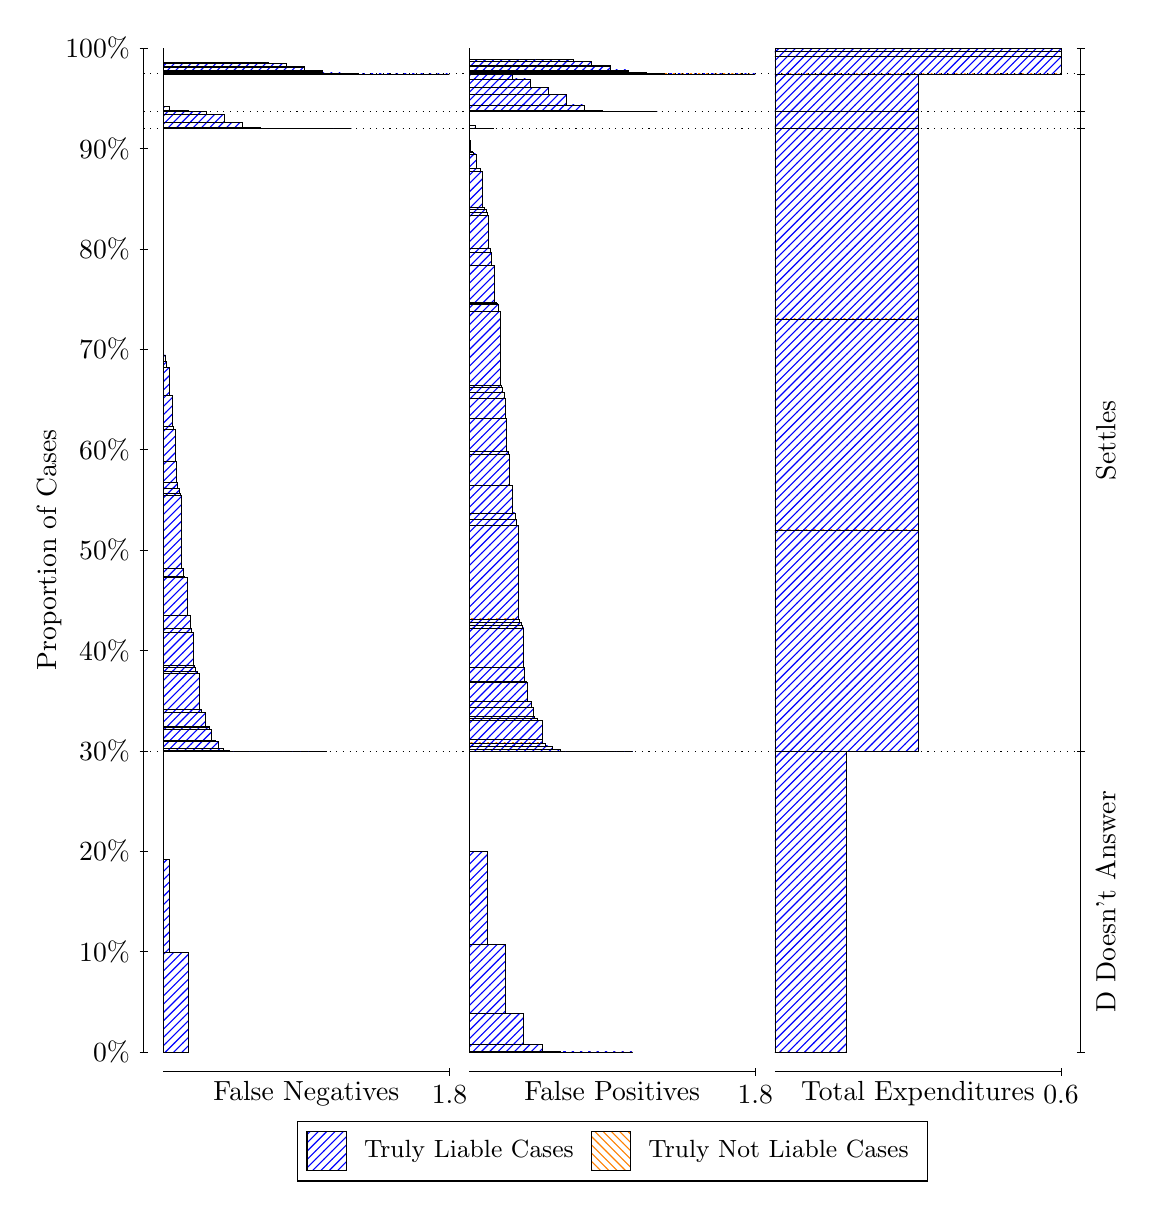
\begin{tikzpicture}
\draw[black, very thin] (1.5,1.75) -- (1.5,14.5);
\node[rotate=90, anchor=center] at (0.3, 8.125) {Proportion of Cases};
\draw[black, very thin] (1.45,1.75) -- (1.55,1.75);
\node[anchor=east] at (1.45, 1.75) {0\%};
\draw[black, very thin] (1.45,3.025) -- (1.55,3.025);
\node[anchor=east] at (1.45, 3.025) {10\%};
\draw[black, very thin] (1.45,4.3) -- (1.55,4.3);
\node[anchor=east] at (1.45, 4.3) {20\%};
\draw[black, very thin] (1.45,5.575) -- (1.55,5.575);
\node[anchor=east] at (1.45, 5.575) {30\%};
\draw[black, very thin] (1.45,6.85) -- (1.55,6.85);
\node[anchor=east] at (1.45, 6.85) {40\%};
\draw[black, very thin] (1.45,8.125) -- (1.55,8.125);
\node[anchor=east] at (1.45, 8.125) {50\%};
\draw[black, very thin] (1.45,9.4) -- (1.55,9.4);
\node[anchor=east] at (1.45, 9.4) {60\%};
\draw[black, very thin] (1.45,10.675) -- (1.55,10.675);
\node[anchor=east] at (1.45, 10.675) {70\%};
\draw[black, very thin] (1.45,11.95) -- (1.55,11.95);
\node[anchor=east] at (1.45, 11.95) {80\%};
\draw[black, very thin] (1.45,13.225) -- (1.55,13.225);
\node[anchor=east] at (1.45, 13.225) {90\%};
\draw[black, very thin] (1.45,14.5) -- (1.55,14.5);
\node[anchor=east] at (1.45, 14.5) {100\%};

\draw[black, very thin] (13.4,1.75) -- (13.4,14.5);
\draw[black, very thin] (13.35,1.75) -- (13.45,1.75);
\node[anchor=west] at (13.35, 1.75) {};
\draw[black, very thin] (13.35,5.5631) -- (13.45,5.5631);
\node[anchor=west] at (13.35, 5.5631) {};
\draw[black, very thin] (13.35,13.477) -- (13.45,13.477);
\node[anchor=west] at (13.35, 13.477) {};
\draw[black, very thin] (13.35,13.696) -- (13.45,13.696);
\node[anchor=west] at (13.35, 13.696) {};
\draw[black, very thin] (13.35,14.171) -- (13.45,14.171);
\node[anchor=west] at (13.35, 14.171) {};
\draw[black, very thin] (13.35,14.5) -- (13.45,14.5);
\node[anchor=west] at (13.35, 14.5) {};

\draw[black, very thin, pattern color=blue, pattern=north east lines] (1.75,1.75) rectangle (2.0614,3.0136);
\draw[black, very thin, pattern color=blue, pattern=north east lines] (1.75,3.0136) rectangle (1.8307,4.1973);
\draw[black, very thin, pattern color=orange, pattern=north west lines] (1.75,4.1973) rectangle (1.75,4.1973);
\draw[black, very thin, pattern color=blue, pattern=north east lines] (1.75,4.1973) rectangle (1.75,5.5631);
\draw[black, very thin, pattern color=blue, pattern=north east lines] (1.75,5.5631) rectangle (3.8262,5.5631);
\draw[black, very thin, pattern color=blue, pattern=north east lines] (1.75,5.5631) rectangle (3.7224,5.5631);
\draw[black, very thin, pattern color=blue, pattern=north east lines] (1.75,5.5631) rectangle (3.6186,5.5631);
\draw[black, very thin, pattern color=blue, pattern=north east lines] (1.75,5.5631) rectangle (3.5955,5.5631);
\draw[black, very thin, pattern color=blue, pattern=north east lines] (1.75,5.5631) rectangle (3.5148,5.5631);
\draw[black, very thin, pattern color=blue, pattern=north east lines] (1.75,5.5631) rectangle (3.4917,5.5631);
\draw[black, very thin, pattern color=blue, pattern=north east lines] (1.75,5.5631) rectangle (3.411,5.5631);
\draw[black, very thin, pattern color=blue, pattern=north east lines] (1.75,5.5631) rectangle (3.3879,5.5631);
\draw[black, very thin, pattern color=blue, pattern=north east lines] (1.75,5.5631) rectangle (3.3648,5.5631);
\draw[black, very thin, pattern color=blue, pattern=north east lines] (1.75,5.5631) rectangle (3.3071,5.5631);
\draw[black, very thin, pattern color=blue, pattern=north east lines] (1.75,5.5631) rectangle (3.2841,5.5631);
\draw[black, very thin, pattern color=blue, pattern=north east lines] (1.75,5.5631) rectangle (3.261,5.5631);
\draw[black, very thin, pattern color=blue, pattern=north east lines] (1.75,5.5631) rectangle (3.2033,5.5631);
\draw[black, very thin, pattern color=blue, pattern=north east lines] (1.75,5.5631) rectangle (3.1803,5.5631);
\draw[black, very thin, pattern color=blue, pattern=north east lines] (1.75,5.5631) rectangle (3.1572,5.5631);
\draw[black, very thin, pattern color=blue, pattern=north east lines] (1.75,5.5631) rectangle (3.1341,5.5631);
\draw[black, very thin, pattern color=blue, pattern=north east lines] (1.75,5.5631) rectangle (3.0995,5.5631);
\draw[black, very thin, pattern color=blue, pattern=north east lines] (1.75,5.5631) rectangle (3.0765,5.5631);
\draw[black, very thin, pattern color=blue, pattern=north east lines] (1.75,5.5631) rectangle (3.0534,5.5631);
\draw[black, very thin, pattern color=blue, pattern=north east lines] (1.75,5.5631) rectangle (3.0303,5.5631);
\draw[black, very thin, pattern color=blue, pattern=north east lines] (1.75,5.5631) rectangle (2.9957,5.5631);
\draw[black, very thin, pattern color=blue, pattern=north east lines] (1.75,5.5631) rectangle (2.9726,5.5631);
\draw[black, very thin, pattern color=blue, pattern=north east lines] (1.75,5.5631) rectangle (2.9496,5.5631);
\draw[black, very thin, pattern color=blue, pattern=north east lines] (1.75,5.5631) rectangle (2.9265,5.5631);
\draw[black, very thin, pattern color=blue, pattern=north east lines] (1.75,5.5631) rectangle (2.9034,5.5632);
\draw[black, very thin, pattern color=blue, pattern=north east lines] (1.75,5.5632) rectangle (2.8919,5.5632);
\draw[black, very thin, pattern color=blue, pattern=north east lines] (1.75,5.5632) rectangle (2.8688,5.5632);
\draw[black, very thin, pattern color=blue, pattern=north east lines] (1.75,5.5632) rectangle (2.8458,5.5632);
\draw[black, very thin, pattern color=blue, pattern=north east lines] (1.75,5.5632) rectangle (2.8227,5.5634);
\draw[black, very thin, pattern color=blue, pattern=north east lines] (1.75,5.5634) rectangle (2.7996,5.5634);
\draw[black, very thin, pattern color=blue, pattern=north east lines] (1.75,5.5634) rectangle (2.7881,5.5634);
\draw[black, very thin, pattern color=blue, pattern=north east lines] (1.75,5.5634) rectangle (2.765,5.5634);
\draw[black, very thin, pattern color=blue, pattern=north east lines] (1.75,5.5634) rectangle (2.742,5.5638);
\draw[black, very thin, pattern color=blue, pattern=north east lines] (1.75,5.5638) rectangle (2.7189,5.5638);
\draw[black, very thin, pattern color=blue, pattern=north east lines] (1.75,5.5638) rectangle (2.6958,5.5638);
\draw[black, very thin, pattern color=blue, pattern=north east lines] (1.75,5.5638) rectangle (2.6728,5.5703);
\draw[black, very thin, pattern color=blue, pattern=north east lines] (1.75,5.5703) rectangle (2.6612,5.5703);
\draw[black, very thin, pattern color=blue, pattern=north east lines] (1.75,5.5703) rectangle (2.6381,5.5703);
\draw[black, very thin, pattern color=blue, pattern=north east lines] (1.75,5.5703) rectangle (2.6151,5.5705);
\draw[black, very thin, pattern color=blue, pattern=north east lines] (1.75,5.5705) rectangle (2.592,5.5829);
\draw[black, very thin, pattern color=blue, pattern=north east lines] (1.75,5.5829) rectangle (2.5805,5.5829);
\draw[black, very thin, pattern color=blue, pattern=north east lines] (1.75,5.5829) rectangle (2.5689,5.5846);
\draw[black, very thin, pattern color=blue, pattern=north east lines] (1.75,5.5846) rectangle (2.5574,5.585);
\draw[black, very thin, pattern color=blue, pattern=north east lines] (1.75,5.585) rectangle (2.5343,5.585);
\draw[black, very thin, pattern color=blue, pattern=north east lines] (1.75,5.585) rectangle (2.5113,5.6016);
\draw[black, very thin, pattern color=blue, pattern=north east lines] (1.75,5.6016) rectangle (2.4882,5.6016);
\draw[black, very thin, pattern color=blue, pattern=north east lines] (1.75,5.6016) rectangle (2.4767,5.6016);
\draw[black, very thin, pattern color=blue, pattern=north east lines] (1.75,5.6016) rectangle (2.4651,5.605);
\draw[black, very thin, pattern color=blue, pattern=north east lines] (1.75,5.605) rectangle (2.4421,5.7012);
\draw[black, very thin, pattern color=blue, pattern=north east lines] (1.75,5.7012) rectangle (2.4305,5.7012);
\draw[black, very thin, pattern color=blue, pattern=north east lines] (1.75,5.7012) rectangle (2.4075,5.7036);
\draw[black, very thin, pattern color=blue, pattern=north east lines] (1.75,5.7036) rectangle (2.3844,5.7085);
\draw[black, very thin, pattern color=blue, pattern=north east lines] (1.75,5.7085) rectangle (2.3729,5.7103);
\draw[black, very thin, pattern color=blue, pattern=north east lines] (1.75,5.7103) rectangle (2.3613,5.8493);
\draw[black, very thin, pattern color=blue, pattern=north east lines] (1.75,5.8493) rectangle (2.3498,5.8493);
\draw[black, very thin, pattern color=blue, pattern=north east lines] (1.75,5.8493) rectangle (2.3383,5.8678);
\draw[black, very thin, pattern color=blue, pattern=north east lines] (1.75,5.8678) rectangle (2.3267,5.8846);
\draw[black, very thin, pattern color=blue, pattern=north east lines] (1.75,5.8846) rectangle (2.3037,5.8846);
\draw[black, very thin, pattern color=blue, pattern=north east lines] (1.75,5.8846) rectangle (2.2806,6.0649);
\draw[black, very thin, pattern color=blue, pattern=north east lines] (1.75,6.0649) rectangle (2.2575,6.0659);
\draw[black, very thin, pattern color=blue, pattern=north east lines] (1.75,6.0659) rectangle (2.246,6.0662);
\draw[black, very thin, pattern color=blue, pattern=north east lines] (1.75,6.0662) rectangle (2.2344,6.1031);
\draw[black, very thin, pattern color=blue, pattern=north east lines] (1.75,6.1031) rectangle (2.2114,6.5588);
\draw[black, very thin, pattern color=blue, pattern=north east lines] (1.75,6.5588) rectangle (2.1998,6.5612);
\draw[black, very thin, pattern color=blue, pattern=north east lines] (1.75,6.5612) rectangle (2.1768,6.5886);
\draw[black, very thin, pattern color=blue, pattern=north east lines] (1.75,6.5886) rectangle (2.1537,6.6306);
\draw[black, very thin, pattern color=blue, pattern=north east lines] (1.75,6.6306) rectangle (2.1422,6.666);
\draw[black, very thin, pattern color=blue, pattern=north east lines] (1.75,6.666) rectangle (2.1306,7.0803);
\draw[black, very thin, pattern color=blue, pattern=north east lines] (1.75,7.0803) rectangle (2.1191,7.0803);
\draw[black, very thin, pattern color=blue, pattern=north east lines] (1.75,7.0803) rectangle (2.1076,7.129);
\draw[black, very thin, pattern color=blue, pattern=north east lines] (1.75,7.129) rectangle (2.096,7.2967);
\draw[black, very thin, pattern color=blue, pattern=north east lines] (1.75,7.2967) rectangle (2.073,7.297);
\draw[black, very thin, pattern color=blue, pattern=north east lines] (1.75,7.297) rectangle (2.0499,7.7754);
\draw[black, very thin, pattern color=blue, pattern=north east lines] (1.75,7.7754) rectangle (2.0268,7.7819);
\draw[black, very thin, pattern color=blue, pattern=north east lines] (1.75,7.7819) rectangle (2.0153,7.7911);
\draw[black, very thin, pattern color=blue, pattern=north east lines] (1.75,7.7911) rectangle (2.0038,7.8883);
\draw[black, very thin, pattern color=blue, pattern=north east lines] (1.75,7.8883) rectangle (1.9807,8.8224);
\draw[black, very thin, pattern color=blue, pattern=north east lines] (1.75,8.8224) rectangle (1.9692,8.8457);
\draw[black, very thin, pattern color=blue, pattern=north east lines] (1.75,8.8457) rectangle (1.9461,8.9146);
\draw[black, very thin, pattern color=blue, pattern=north east lines] (1.75,8.9146) rectangle (1.923,8.9877);
\draw[black, very thin, pattern color=blue, pattern=north east lines] (1.75,8.9877) rectangle (1.9115,9.2464);
\draw[black, very thin, pattern color=blue, pattern=north east lines] (1.75,9.2464) rectangle (1.8999,9.6562);
\draw[black, very thin, pattern color=blue, pattern=north east lines] (1.75,9.6562) rectangle (1.8884,9.6568);
\draw[black, very thin, pattern color=blue, pattern=north east lines] (1.75,9.6568) rectangle (1.8769,9.6959);
\draw[black, very thin, pattern color=blue, pattern=north east lines] (1.75,9.6959) rectangle (1.8653,10.09);
\draw[black, very thin, pattern color=blue, pattern=north east lines] (1.75,10.09) rectangle (1.8423,10.092);
\draw[black, very thin, pattern color=blue, pattern=north east lines] (1.75,10.092) rectangle (1.8192,10.444);
\draw[black, very thin, pattern color=blue, pattern=north east lines] (1.75,10.444) rectangle (1.7961,10.451);
\draw[black, very thin, pattern color=blue, pattern=north east lines] (1.75,10.451) rectangle (1.7846,10.526);
\draw[black, very thin, pattern color=blue, pattern=north east lines] (1.75,10.526) rectangle (1.7731,10.604);
\draw[black, very thin, pattern color=orange, pattern=north west lines] (1.75,10.604) rectangle (1.75,10.604);
\draw[black, very thin, pattern color=blue, pattern=north east lines] (1.75,10.604) rectangle (1.75,13.477);
\draw[black, very thin, pattern color=blue, pattern=north east lines] (1.75,13.477) rectangle (4.1376,13.477);
\draw[black, very thin, pattern color=blue, pattern=north east lines] (1.75,13.477) rectangle (3.9069,13.477);
\draw[black, very thin, pattern color=blue, pattern=north east lines] (1.75,13.477) rectangle (3.6762,13.477);
\draw[black, very thin, pattern color=blue, pattern=north east lines] (1.75,13.477) rectangle (3.4456,13.477);
\draw[black, very thin, pattern color=blue, pattern=north east lines] (1.75,13.477) rectangle (3.2149,13.477);
\draw[black, very thin, pattern color=blue, pattern=north east lines] (1.75,13.477) rectangle (2.9842,13.488);
\draw[black, very thin, pattern color=blue, pattern=north east lines] (1.75,13.488) rectangle (2.7535,13.555);
\draw[black, very thin, pattern color=blue, pattern=north east lines] (1.75,13.555) rectangle (2.5228,13.653);
\draw[black, very thin, pattern color=blue, pattern=north east lines] (1.75,13.653) rectangle (2.2921,13.691);
\draw[black, very thin, pattern color=blue, pattern=north east lines] (1.75,13.691) rectangle (2.0614,13.696);
\draw[black, very thin, pattern color=orange, pattern=north west lines] (1.75,13.696) rectangle (1.75,13.696);
\draw[black, very thin, pattern color=blue, pattern=north east lines] (1.75,13.696) rectangle (2.0614,13.706);
\draw[black, very thin, pattern color=blue, pattern=north east lines] (1.75,13.706) rectangle (1.8307,13.76);
\draw[black, very thin, pattern color=orange, pattern=north west lines] (1.75,13.76) rectangle (1.75,13.76);
\draw[black, very thin, pattern color=blue, pattern=north east lines] (1.75,13.76) rectangle (1.75,14.171);
\draw[black, very thin, pattern color=blue, pattern=north east lines] (1.75,14.171) rectangle (5.3833,14.171);
\draw[black, very thin, pattern color=blue, pattern=north east lines] (1.75,14.171) rectangle (5.1526,14.171);
\draw[black, very thin, pattern color=blue, pattern=north east lines] (1.75,14.171) rectangle (4.922,14.171);
\draw[black, very thin, pattern color=blue, pattern=north east lines] (1.75,14.171) rectangle (4.6913,14.171);
\draw[black, very thin, pattern color=blue, pattern=north east lines] (1.75,14.171) rectangle (4.6913,14.171);
\draw[black, very thin, pattern color=blue, pattern=north east lines] (1.75,14.171) rectangle (4.4606,14.171);
\draw[black, very thin, pattern color=blue, pattern=north east lines] (1.75,14.171) rectangle (4.4606,14.171);
\draw[black, very thin, pattern color=blue, pattern=north east lines] (1.75,14.171) rectangle (4.2299,14.173);
\draw[black, very thin, pattern color=blue, pattern=north east lines] (1.75,14.173) rectangle (3.9992,14.175);
\draw[black, very thin, pattern color=blue, pattern=north east lines] (1.75,14.175) rectangle (3.9992,14.183);
\draw[black, very thin, pattern color=blue, pattern=north east lines] (1.75,14.183) rectangle (3.7685,14.188);
\draw[black, very thin, pattern color=blue, pattern=north east lines] (1.75,14.188) rectangle (3.7685,14.205);
\draw[black, very thin, pattern color=blue, pattern=north east lines] (1.75,14.205) rectangle (3.7685,14.216);
\draw[black, very thin, pattern color=blue, pattern=north east lines] (1.75,14.216) rectangle (3.5378,14.254);
\draw[black, very thin, pattern color=blue, pattern=north east lines] (1.75,14.254) rectangle (3.5378,14.266);
\draw[black, very thin, pattern color=blue, pattern=north east lines] (1.75,14.266) rectangle (3.3071,14.303);
\draw[black, very thin, pattern color=blue, pattern=north east lines] (1.75,14.303) rectangle (3.0765,14.305);
\draw[black, very thin, pattern color=blue, pattern=north east lines] (1.75,14.305) rectangle (3.0765,14.313);
\draw[black, very thin, pattern color=blue, pattern=north east lines] (1.75,14.313) rectangle (3.0534,14.313);
\draw[black, very thin, pattern color=blue, pattern=north east lines] (1.75,14.313) rectangle (2.8458,14.313);
\draw[black, very thin, pattern color=blue, pattern=north east lines] (1.75,14.313) rectangle (2.8458,14.313);
\draw[black, very thin, pattern color=blue, pattern=north east lines] (1.75,14.313) rectangle (2.8227,14.313);
\draw[black, very thin, pattern color=blue, pattern=north east lines] (1.75,14.313) rectangle (2.8227,14.313);
\draw[black, very thin, pattern color=blue, pattern=north east lines] (1.75,14.313) rectangle (2.6151,14.313);
\draw[black, very thin, pattern color=blue, pattern=north east lines] (1.75,14.313) rectangle (2.6151,14.313);
\draw[black, very thin, pattern color=blue, pattern=north east lines] (1.75,14.313) rectangle (2.592,14.313);
\draw[black, very thin, pattern color=blue, pattern=north east lines] (1.75,14.313) rectangle (2.592,14.313);
\draw[black, very thin, pattern color=blue, pattern=north east lines] (1.75,14.313) rectangle (2.592,14.313);
\draw[black, very thin, pattern color=blue, pattern=north east lines] (1.75,14.313) rectangle (2.3844,14.313);
\draw[black, very thin, pattern color=blue, pattern=north east lines] (1.75,14.313) rectangle (2.3844,14.313);
\draw[black, very thin, pattern color=blue, pattern=north east lines] (1.75,14.313) rectangle (2.3613,14.313);
\draw[black, very thin, pattern color=blue, pattern=north east lines] (1.75,14.313) rectangle (2.3613,14.313);
\draw[black, very thin, pattern color=blue, pattern=north east lines] (1.75,14.313) rectangle (2.1537,14.313);
\draw[black, very thin, pattern color=blue, pattern=north east lines] (1.75,14.313) rectangle (2.1537,14.313);
\draw[black, very thin, pattern color=blue, pattern=north east lines] (1.75,14.313) rectangle (2.1306,14.313);
\draw[black, very thin, pattern color=blue, pattern=north east lines] (1.75,14.313) rectangle (2.1306,14.313);
\draw[black, very thin, pattern color=blue, pattern=north east lines] (1.75,14.313) rectangle (2.1306,14.313);
\draw[black, very thin, pattern color=blue, pattern=north east lines] (1.75,14.313) rectangle (1.923,14.313);
\draw[black, very thin, pattern color=blue, pattern=north east lines] (1.75,14.313) rectangle (1.923,14.313);
\draw[black, very thin, pattern color=blue, pattern=north east lines] (1.75,14.313) rectangle (1.8999,14.314);
\draw[black, very thin, pattern color=blue, pattern=north east lines] (1.75,14.314) rectangle (1.8999,14.316);
\draw[black, very thin, pattern color=blue, pattern=north east lines] (1.75,14.316) rectangle (1.8999,14.316);
\draw[black, very thin, pattern color=orange, pattern=north west lines] (1.75,14.316) rectangle (1.75,14.316);
\draw[black, very thin, pattern color=blue, pattern=north east lines] (1.75,14.316) rectangle (1.75,14.5);
\draw[black, very thin, pattern color=orange, pattern=north west lines] (5.6333,1.75) rectangle (7.7095,1.75);
\draw[black, very thin, pattern color=blue, pattern=north east lines] (5.6333,1.75) rectangle (7.7095,1.75);
\draw[black, very thin, pattern color=blue, pattern=north east lines] (5.6333,1.75) rectangle (7.4788,1.75);
\draw[black, very thin, pattern color=blue, pattern=north east lines] (5.6333,1.75) rectangle (7.2481,1.75);
\draw[black, very thin, pattern color=blue, pattern=north east lines] (5.6333,1.75) rectangle (7.0175,1.7503);
\draw[black, very thin, pattern color=blue, pattern=north east lines] (5.6333,1.7503) rectangle (6.7868,1.7582);
\draw[black, very thin, pattern color=blue, pattern=north east lines] (5.6333,1.7582) rectangle (6.5561,1.8434);
\draw[black, very thin, pattern color=blue, pattern=north east lines] (5.6333,1.8434) rectangle (6.3254,2.2366);
\draw[black, very thin, pattern color=blue, pattern=north east lines] (5.6333,2.2366) rectangle (6.0947,3.1157);
\draw[black, very thin, pattern color=blue, pattern=north east lines] (5.6333,3.1157) rectangle (5.864,4.2995);
\draw[black, very thin, pattern color=blue, pattern=north east lines] (5.6333,4.2995) rectangle (5.6333,5.5631);
\draw[black, very thin, pattern color=orange, pattern=north west lines] (5.6333,5.5631) rectangle (7.7095,5.5631);
\draw[black, very thin, pattern color=blue, pattern=north east lines] (5.6333,5.5631) rectangle (7.7095,5.5631);
\draw[black, very thin, pattern color=orange, pattern=north west lines] (5.6333,5.5631) rectangle (7.6057,5.5631);
\draw[black, very thin, pattern color=blue, pattern=north east lines] (5.6333,5.5631) rectangle (7.6057,5.5631);
\draw[black, very thin, pattern color=orange, pattern=north west lines] (5.6333,5.5631) rectangle (7.5019,5.5631);
\draw[black, very thin, pattern color=blue, pattern=north east lines] (5.6333,5.5631) rectangle (7.5019,5.5631);
\draw[black, very thin, pattern color=blue, pattern=north east lines] (5.6333,5.5631) rectangle (7.4788,5.5631);
\draw[black, very thin, pattern color=blue, pattern=north east lines] (5.6333,5.5631) rectangle (7.375,5.5631);
\draw[black, very thin, pattern color=orange, pattern=north west lines] (5.6333,5.5631) rectangle (7.2943,5.5631);
\draw[black, very thin, pattern color=blue, pattern=north east lines] (5.6333,5.5631) rectangle (7.2943,5.5631);
\draw[black, very thin, pattern color=blue, pattern=north east lines] (5.6333,5.5631) rectangle (7.2712,5.5631);
\draw[black, very thin, pattern color=blue, pattern=north east lines] (5.6333,5.5631) rectangle (7.2481,5.5631);
\draw[black, very thin, pattern color=orange, pattern=north west lines] (5.6333,5.5631) rectangle (7.1905,5.5631);
\draw[black, very thin, pattern color=blue, pattern=north east lines] (5.6333,5.5631) rectangle (7.1905,5.5631);
\draw[black, very thin, pattern color=blue, pattern=north east lines] (5.6333,5.5631) rectangle (7.1443,5.5631);
\draw[black, very thin, pattern color=orange, pattern=north west lines] (5.6333,5.5631) rectangle (7.0867,5.5631);
\draw[black, very thin, pattern color=blue, pattern=north east lines] (5.6333,5.5631) rectangle (7.0867,5.5631);
\draw[black, very thin, pattern color=blue, pattern=north east lines] (5.6333,5.5631) rectangle (7.0636,5.5631);
\draw[black, very thin, pattern color=blue, pattern=north east lines] (5.6333,5.5631) rectangle (7.0405,5.5631);
\draw[black, very thin, pattern color=blue, pattern=north east lines] (5.6333,5.5631) rectangle (7.0175,5.5636);
\draw[black, very thin, pattern color=orange, pattern=north west lines] (5.6333,5.5636) rectangle (6.9829,5.5636);
\draw[black, very thin, pattern color=blue, pattern=north east lines] (5.6333,5.5636) rectangle (6.9829,5.5636);
\draw[black, very thin, pattern color=blue, pattern=north east lines] (5.6333,5.5636) rectangle (6.9598,5.5637);
\draw[black, very thin, pattern color=blue, pattern=north east lines] (5.6333,5.5637) rectangle (6.9137,5.5657);
\draw[black, very thin, pattern color=orange, pattern=north west lines] (5.6333,5.5657) rectangle (6.879,5.5657);
\draw[black, very thin, pattern color=blue, pattern=north east lines] (5.6333,5.5657) rectangle (6.879,5.5658);
\draw[black, very thin, pattern color=blue, pattern=north east lines] (5.6333,5.5658) rectangle (6.856,5.5658);
\draw[black, very thin, pattern color=blue, pattern=north east lines] (5.6333,5.5658) rectangle (6.8329,5.5669);
\draw[black, very thin, pattern color=blue, pattern=north east lines] (5.6333,5.5669) rectangle (6.8098,5.5675);
\draw[black, very thin, pattern color=blue, pattern=north east lines] (5.6333,5.5675) rectangle (6.7868,5.5932);
\draw[black, very thin, pattern color=orange, pattern=north west lines] (5.6333,5.5932) rectangle (6.7752,5.5932);
\draw[black, very thin, pattern color=blue, pattern=north east lines] (5.6333,5.5932) rectangle (6.7752,5.5933);
\draw[black, very thin, pattern color=blue, pattern=north east lines] (5.6333,5.5933) rectangle (6.7522,5.5936);
\draw[black, very thin, pattern color=blue, pattern=north east lines] (5.6333,5.5936) rectangle (6.7291,5.5949);
\draw[black, very thin, pattern color=blue, pattern=north east lines] (5.6333,5.5949) rectangle (6.683,5.6311);
\draw[black, very thin, pattern color=orange, pattern=north west lines] (5.6333,5.6311) rectangle (6.6714,5.6311);
\draw[black, very thin, pattern color=blue, pattern=north east lines] (5.6333,5.6311) rectangle (6.6714,5.6311);
\draw[black, very thin, pattern color=blue, pattern=north east lines] (5.6333,5.6311) rectangle (6.6484,5.6365);
\draw[black, very thin, pattern color=blue, pattern=north east lines] (5.6333,5.6365) rectangle (6.6253,5.6368);
\draw[black, very thin, pattern color=blue, pattern=north east lines] (5.6333,5.6368) rectangle (6.6022,5.6707);
\draw[black, very thin, pattern color=blue, pattern=north east lines] (5.6333,5.6707) rectangle (6.5792,5.6744);
\draw[black, very thin, pattern color=orange, pattern=north west lines] (5.6333,5.6744) rectangle (6.5676,5.6744);
\draw[black, very thin, pattern color=blue, pattern=north east lines] (5.6333,5.6744) rectangle (6.5676,5.715);
\draw[black, very thin, pattern color=blue, pattern=north east lines] (5.6333,5.715) rectangle (6.5561,5.9566);
\draw[black, very thin, pattern color=blue, pattern=north east lines] (5.6333,5.9566) rectangle (6.5446,5.9591);
\draw[black, very thin, pattern color=blue, pattern=north east lines] (5.6333,5.9591) rectangle (6.5215,5.9655);
\draw[black, very thin, pattern color=blue, pattern=north east lines] (5.6333,5.9655) rectangle (6.4984,5.9828);
\draw[black, very thin, pattern color=orange, pattern=north west lines] (5.6333,5.9828) rectangle (6.4638,5.9828);
\draw[black, very thin, pattern color=blue, pattern=north east lines] (5.6333,5.9828) rectangle (6.4638,6.0102);
\draw[black, very thin, pattern color=blue, pattern=north east lines] (5.6333,6.0102) rectangle (6.4523,6.1285);
\draw[black, very thin, pattern color=blue, pattern=north east lines] (5.6333,6.1285) rectangle (6.4407,6.1297);
\draw[black, very thin, pattern color=blue, pattern=north east lines] (5.6333,6.1297) rectangle (6.4177,6.2066);
\draw[black, very thin, pattern color=blue, pattern=north east lines] (5.6333,6.2066) rectangle (6.3946,6.2088);
\draw[black, very thin, pattern color=blue, pattern=north east lines] (5.6333,6.2088) rectangle (6.3715,6.4425);
\draw[black, very thin, pattern color=orange, pattern=north west lines] (5.6333,6.4425) rectangle (6.36,6.4425);
\draw[black, very thin, pattern color=blue, pattern=north east lines] (5.6333,6.4425) rectangle (6.36,6.4563);
\draw[black, very thin, pattern color=blue, pattern=north east lines] (5.6333,6.4563) rectangle (6.3485,6.46);
\draw[black, very thin, pattern color=blue, pattern=north east lines] (5.6333,6.46) rectangle (6.3369,6.6298);
\draw[black, very thin, pattern color=blue, pattern=north east lines] (5.6333,6.6298) rectangle (6.3254,7.1352);
\draw[black, very thin, pattern color=blue, pattern=north east lines] (5.6333,7.1352) rectangle (6.3139,7.163);
\draw[black, very thin, pattern color=blue, pattern=north east lines] (5.6333,7.163) rectangle (6.2908,7.2043);
\draw[black, very thin, pattern color=blue, pattern=north east lines] (5.6333,7.2043) rectangle (6.2677,7.2492);
\draw[black, very thin, pattern color=orange, pattern=north west lines] (5.6333,7.2492) rectangle (6.2562,7.2492);
\draw[black, very thin, pattern color=blue, pattern=north east lines] (5.6333,7.2492) rectangle (6.2562,8.4361);
\draw[black, very thin, pattern color=blue, pattern=north east lines] (5.6333,8.4361) rectangle (6.2331,8.5142);
\draw[black, very thin, pattern color=blue, pattern=north east lines] (5.6333,8.5142) rectangle (6.2216,8.5889);
\draw[black, very thin, pattern color=blue, pattern=north east lines] (5.6333,8.5889) rectangle (6.2101,8.5955);
\draw[black, very thin, pattern color=blue, pattern=north east lines] (5.6333,8.5955) rectangle (6.187,8.9475);
\draw[black, very thin, pattern color=blue, pattern=north east lines] (5.6333,8.9475) rectangle (6.1639,8.9497);
\draw[black, very thin, pattern color=blue, pattern=north east lines] (5.6333,8.9497) rectangle (6.1408,9.344);
\draw[black, very thin, pattern color=blue, pattern=north east lines] (5.6333,9.344) rectangle (6.1293,9.3831);
\draw[black, very thin, pattern color=blue, pattern=north east lines] (5.6333,9.3831) rectangle (6.1178,9.3837);
\draw[black, very thin, pattern color=blue, pattern=north east lines] (5.6333,9.3837) rectangle (6.1062,9.7935);
\draw[black, very thin, pattern color=blue, pattern=north east lines] (5.6333,9.7935) rectangle (6.0947,10.052);
\draw[black, very thin, pattern color=blue, pattern=north east lines] (5.6333,10.052) rectangle (6.0832,10.125);
\draw[black, very thin, pattern color=blue, pattern=north east lines] (5.6333,10.125) rectangle (6.0601,10.194);
\draw[black, very thin, pattern color=blue, pattern=north east lines] (5.6333,10.194) rectangle (6.037,10.217);
\draw[black, very thin, pattern color=blue, pattern=north east lines] (5.6333,10.217) rectangle (6.0255,11.152);
\draw[black, very thin, pattern color=blue, pattern=north east lines] (5.6333,11.152) rectangle (6.0024,11.249);
\draw[black, very thin, pattern color=blue, pattern=north east lines] (5.6333,11.249) rectangle (5.9909,11.258);
\draw[black, very thin, pattern color=blue, pattern=north east lines] (5.6333,11.258) rectangle (5.9794,11.265);
\draw[black, very thin, pattern color=blue, pattern=north east lines] (5.6333,11.265) rectangle (5.9563,11.743);
\draw[black, very thin, pattern color=blue, pattern=north east lines] (5.6333,11.743) rectangle (5.9332,11.743);
\draw[black, very thin, pattern color=blue, pattern=north east lines] (5.6333,11.743) rectangle (5.9102,11.911);
\draw[black, very thin, pattern color=blue, pattern=north east lines] (5.6333,11.911) rectangle (5.8986,11.96);
\draw[black, very thin, pattern color=blue, pattern=north east lines] (5.6333,11.96) rectangle (5.8871,11.96);
\draw[black, very thin, pattern color=blue, pattern=north east lines] (5.6333,11.96) rectangle (5.8756,12.374);
\draw[black, very thin, pattern color=blue, pattern=north east lines] (5.6333,12.374) rectangle (5.864,12.409);
\draw[black, very thin, pattern color=blue, pattern=north east lines] (5.6333,12.409) rectangle (5.8525,12.451);
\draw[black, very thin, pattern color=blue, pattern=north east lines] (5.6333,12.451) rectangle (5.8294,12.479);
\draw[black, very thin, pattern color=blue, pattern=north east lines] (5.6333,12.479) rectangle (5.8063,12.481);
\draw[black, very thin, pattern color=blue, pattern=north east lines] (5.6333,12.481) rectangle (5.7948,12.937);
\draw[black, very thin, pattern color=blue, pattern=north east lines] (5.6333,12.937) rectangle (5.7717,12.974);
\draw[black, very thin, pattern color=blue, pattern=north east lines] (5.6333,12.974) rectangle (5.7602,12.974);
\draw[black, very thin, pattern color=blue, pattern=north east lines] (5.6333,12.974) rectangle (5.7487,12.975);
\draw[black, very thin, pattern color=blue, pattern=north east lines] (5.6333,12.975) rectangle (5.7256,13.155);
\draw[black, very thin, pattern color=blue, pattern=north east lines] (5.6333,13.155) rectangle (5.7025,13.155);
\draw[black, very thin, pattern color=blue, pattern=north east lines] (5.6333,13.155) rectangle (5.6795,13.172);
\draw[black, very thin, pattern color=blue, pattern=north east lines] (5.6333,13.172) rectangle (5.6679,13.191);
\draw[black, very thin, pattern color=blue, pattern=north east lines] (5.6333,13.191) rectangle (5.6564,13.191);
\draw[black, very thin, pattern color=blue, pattern=north east lines] (5.6333,13.191) rectangle (5.6449,13.33);
\draw[black, very thin, pattern color=blue, pattern=north east lines] (5.6333,13.33) rectangle (5.6333,13.477);
\draw[black, very thin, pattern color=orange, pattern=north west lines] (5.6333,13.477) rectangle (5.9448,13.477);
\draw[black, very thin, pattern color=blue, pattern=north east lines] (5.6333,13.477) rectangle (5.9448,13.483);
\draw[black, very thin, pattern color=blue, pattern=north east lines] (5.6333,13.483) rectangle (5.7141,13.521);
\draw[black, very thin, pattern color=blue, pattern=north east lines] (5.6333,13.521) rectangle (5.6333,13.696);
\draw[black, very thin, pattern color=orange, pattern=north west lines] (5.6333,13.696) rectangle (8.021,13.696);
\draw[black, very thin, pattern color=blue, pattern=north east lines] (5.6333,13.696) rectangle (8.021,13.696);
\draw[black, very thin, pattern color=blue, pattern=north east lines] (5.6333,13.696) rectangle (7.7903,13.696);
\draw[black, very thin, pattern color=blue, pattern=north east lines] (5.6333,13.696) rectangle (7.5596,13.697);
\draw[black, very thin, pattern color=blue, pattern=north east lines] (5.6333,13.697) rectangle (7.3289,13.705);
\draw[black, very thin, pattern color=blue, pattern=north east lines] (5.6333,13.705) rectangle (7.0982,13.777);
\draw[black, very thin, pattern color=blue, pattern=north east lines] (5.6333,13.777) rectangle (6.8675,13.91);
\draw[black, very thin, pattern color=blue, pattern=north east lines] (5.6333,13.91) rectangle (6.6368,14.005);
\draw[black, very thin, pattern color=blue, pattern=north east lines] (5.6333,14.005) rectangle (6.4061,14.108);
\draw[black, very thin, pattern color=blue, pattern=north east lines] (5.6333,14.108) rectangle (6.1754,14.162);
\draw[black, very thin, pattern color=blue, pattern=north east lines] (5.6333,14.162) rectangle (5.9448,14.171);
\draw[black, very thin, pattern color=orange, pattern=north west lines] (5.6333,14.171) rectangle (9.2667,14.171);
\draw[black, very thin, pattern color=blue, pattern=north east lines] (5.6333,14.171) rectangle (9.2667,14.171);
\draw[black, very thin, pattern color=orange, pattern=north west lines] (5.6333,14.171) rectangle (9.036,14.171);
\draw[black, very thin, pattern color=blue, pattern=north east lines] (5.6333,14.171) rectangle (9.036,14.171);
\draw[black, very thin, pattern color=orange, pattern=north west lines] (5.6333,14.171) rectangle (8.8053,14.171);
\draw[black, very thin, pattern color=blue, pattern=north east lines] (5.6333,14.171) rectangle (8.8053,14.171);
\draw[black, very thin, pattern color=blue, pattern=north east lines] (5.6333,14.171) rectangle (8.5746,14.171);
\draw[black, very thin, pattern color=orange, pattern=north west lines] (5.6333,14.171) rectangle (8.5746,14.171);
\draw[black, very thin, pattern color=blue, pattern=north east lines] (5.6333,14.171) rectangle (8.5746,14.171);
\draw[black, very thin, pattern color=orange, pattern=north west lines] (5.6333,14.171) rectangle (8.3439,14.171);
\draw[black, very thin, pattern color=blue, pattern=north east lines] (5.6333,14.171) rectangle (8.3439,14.171);
\draw[black, very thin, pattern color=blue, pattern=north east lines] (5.6333,14.171) rectangle (8.3439,14.171);
\draw[black, very thin, pattern color=orange, pattern=north west lines] (5.6333,14.171) rectangle (8.1132,14.171);
\draw[black, very thin, pattern color=blue, pattern=north east lines] (5.6333,14.171) rectangle (8.1132,14.174);
\draw[black, very thin, pattern color=blue, pattern=north east lines] (5.6333,14.174) rectangle (8.1132,14.174);
\draw[black, very thin, pattern color=blue, pattern=north east lines] (5.6333,14.174) rectangle (7.8825,14.176);
\draw[black, very thin, pattern color=orange, pattern=north west lines] (5.6333,14.176) rectangle (7.8825,14.176);
\draw[black, very thin, pattern color=blue, pattern=north east lines] (5.6333,14.176) rectangle (7.8825,14.186);
\draw[black, very thin, pattern color=blue, pattern=north east lines] (5.6333,14.186) rectangle (7.6519,14.198);
\draw[black, very thin, pattern color=orange, pattern=north west lines] (5.6333,14.198) rectangle (7.6519,14.198);
\draw[black, very thin, pattern color=blue, pattern=north east lines] (5.6333,14.198) rectangle (7.6519,14.206);
\draw[black, very thin, pattern color=blue, pattern=north east lines] (5.6333,14.206) rectangle (7.6519,14.223);
\draw[black, very thin, pattern color=blue, pattern=north east lines] (5.6333,14.223) rectangle (7.4212,14.263);
\draw[black, very thin, pattern color=blue, pattern=north east lines] (5.6333,14.263) rectangle (7.4212,14.275);
\draw[black, very thin, pattern color=blue, pattern=north east lines] (5.6333,14.275) rectangle (7.4212,14.284);
\draw[black, very thin, pattern color=blue, pattern=north east lines] (5.6333,14.284) rectangle (7.1905,14.332);
\draw[black, very thin, pattern color=blue, pattern=north east lines] (5.6333,14.332) rectangle (7.1905,14.334);
\draw[black, very thin, pattern color=blue, pattern=north east lines] (5.6333,14.334) rectangle (6.9598,14.336);
\draw[black, very thin, pattern color=blue, pattern=north east lines] (5.6333,14.336) rectangle (6.9598,14.355);
\draw[black, very thin, pattern color=blue, pattern=north east lines] (5.6333,14.355) rectangle (6.9598,14.355);
\draw[black, very thin, pattern color=orange, pattern=north west lines] (5.6333,14.355) rectangle (6.9367,14.355);
\draw[black, very thin, pattern color=blue, pattern=north east lines] (5.6333,14.355) rectangle (6.9367,14.355);
\draw[black, very thin, pattern color=blue, pattern=north east lines] (5.6333,14.355) rectangle (6.7291,14.357);
\draw[black, very thin, pattern color=blue, pattern=north east lines] (5.6333,14.357) rectangle (6.7291,14.358);
\draw[black, very thin, pattern color=orange, pattern=north west lines] (5.6333,14.358) rectangle (6.706,14.358);
\draw[black, very thin, pattern color=blue, pattern=north east lines] (5.6333,14.358) rectangle (6.706,14.358);
\draw[black, very thin, pattern color=blue, pattern=north east lines] (5.6333,14.358) rectangle (6.4984,14.358);
\draw[black, very thin, pattern color=blue, pattern=north east lines] (5.6333,14.358) rectangle (6.4984,14.358);
\draw[black, very thin, pattern color=blue, pattern=north east lines] (5.6333,14.358) rectangle (6.4984,14.358);
\draw[black, very thin, pattern color=orange, pattern=north west lines] (5.6333,14.358) rectangle (6.4753,14.358);
\draw[black, very thin, pattern color=blue, pattern=north east lines] (5.6333,14.358) rectangle (6.4753,14.358);
\draw[black, very thin, pattern color=blue, pattern=north east lines] (5.6333,14.358) rectangle (6.4753,14.358);
\draw[black, very thin, pattern color=blue, pattern=north east lines] (5.6333,14.358) rectangle (6.4753,14.358);
\draw[black, very thin, pattern color=blue, pattern=north east lines] (5.6333,14.358) rectangle (6.2677,14.358);
\draw[black, very thin, pattern color=blue, pattern=north east lines] (5.6333,14.358) rectangle (6.2677,14.358);
\draw[black, very thin, pattern color=blue, pattern=north east lines] (5.6333,14.358) rectangle (6.2447,14.358);
\draw[black, very thin, pattern color=orange, pattern=north west lines] (5.6333,14.358) rectangle (6.2447,14.358);
\draw[black, very thin, pattern color=blue, pattern=north east lines] (5.6333,14.358) rectangle (6.2447,14.358);
\draw[black, very thin, pattern color=blue, pattern=north east lines] (5.6333,14.358) rectangle (6.2447,14.358);
\draw[black, very thin, pattern color=blue, pattern=north east lines] (5.6333,14.358) rectangle (6.037,14.358);
\draw[black, very thin, pattern color=blue, pattern=north east lines] (5.6333,14.358) rectangle (6.014,14.358);
\draw[black, very thin, pattern color=orange, pattern=north west lines] (5.6333,14.358) rectangle (6.014,14.358);
\draw[black, very thin, pattern color=blue, pattern=north east lines] (5.6333,14.358) rectangle (6.014,14.358);
\draw[black, very thin, pattern color=blue, pattern=north east lines] (5.6333,14.358) rectangle (6.014,14.358);
\draw[black, very thin, pattern color=blue, pattern=north east lines] (5.6333,14.358) rectangle (5.8063,14.358);
\draw[black, very thin, pattern color=blue, pattern=north east lines] (5.6333,14.358) rectangle (5.8063,14.358);
\draw[black, very thin, pattern color=blue, pattern=north east lines] (5.6333,14.358) rectangle (5.7833,14.358);
\draw[black, very thin, pattern color=orange, pattern=north west lines] (5.6333,14.358) rectangle (5.7833,14.358);
\draw[black, very thin, pattern color=blue, pattern=north east lines] (5.6333,14.358) rectangle (5.7833,14.358);
\draw[black, very thin, pattern color=blue, pattern=north east lines] (5.6333,14.358) rectangle (5.7833,14.359);
\draw[black, very thin, pattern color=orange, pattern=north west lines] (5.6333,14.359) rectangle (5.6333,14.359);
\draw[black, very thin, pattern color=blue, pattern=north east lines] (5.6333,14.359) rectangle (5.6333,14.5);
\draw[black, very thin, pattern color=orange, pattern=north west lines] (9.5167,1.75) rectangle (10.425,1.75);
\draw[black, very thin, pattern color=blue, pattern=north east lines] (9.5167,1.75) rectangle (10.425,5.5631);
\draw[black, very thin, pattern color=orange, pattern=north west lines] (9.5167,5.5631) rectangle (11.333,5.5631);
\draw[black, very thin, pattern color=blue, pattern=north east lines] (9.5167,5.5631) rectangle (11.333,8.3792);
\draw[black, very thin, pattern color=orange, pattern=north west lines] (9.5167,8.3792) rectangle (11.333,8.3792);
\draw[black, very thin, pattern color=blue, pattern=north east lines] (9.5167,8.3792) rectangle (11.333,11.059);
\draw[black, very thin, pattern color=orange, pattern=north west lines] (9.5167,11.059) rectangle (11.333,11.059);
\draw[black, very thin, pattern color=blue, pattern=north east lines] (9.5167,11.059) rectangle (11.333,13.477);
\draw[black, very thin, pattern color=orange, pattern=north west lines] (9.5167,13.477) rectangle (11.333,13.477);
\draw[black, very thin, pattern color=blue, pattern=north east lines] (9.5167,13.477) rectangle (11.333,13.696);
\draw[black, very thin, pattern color=orange, pattern=north west lines] (9.5167,13.696) rectangle (11.333,13.696);
\draw[black, very thin, pattern color=blue, pattern=north east lines] (9.5167,13.696) rectangle (11.333,14.171);
\draw[black, very thin, pattern color=orange, pattern=north west lines] (9.5167,14.171) rectangle (13.15,14.171);
\draw[black, very thin, pattern color=blue, pattern=north east lines] (9.5167,14.171) rectangle (13.15,14.391);
\draw[black, very thin, pattern color=orange, pattern=north west lines] (9.5167,14.391) rectangle (13.15,14.391);
\draw[black, very thin, pattern color=blue, pattern=north east lines] (9.5167,14.391) rectangle (13.15,14.462);
\draw[black, very thin, pattern color=orange, pattern=north west lines] (9.5167,14.462) rectangle (13.15,14.462);
\draw[black, very thin, pattern color=blue, pattern=north east lines] (9.5167,14.462) rectangle (13.15,14.5);
\draw[black, dotted] (1.5,5.5631) -- (13.4,5.5631);
\draw[black, dotted] (1.5,13.477) -- (13.4,13.477);
\draw[black, dotted] (1.5,13.696) -- (13.4,13.696);
\draw[black, dotted] (1.5,14.171) -- (13.4,14.171);
\draw[black, very thin] (1.75,1.5) -- (5.3833,1.5);
\node[anchor=north] at (3.5667, 1.5) {False Negatives};
\draw[black, very thin] (5.3833,1.45) -- (5.3833,1.55);
\node[anchor=north] at (5.3833, 1.45) {1.8};

\draw[black, very thin] (5.6333,1.5) -- (9.2667,1.5);
\node[anchor=north] at (7.45, 1.5) {False Positives};
\draw[black, very thin] (9.2667,1.45) -- (9.2667,1.55);
\node[anchor=north] at (9.2667, 1.45) {1.8};

\draw[black, very thin] (9.5167,1.5) -- (13.15,1.5);
\node[anchor=north] at (11.333, 1.5) {Total Expenditures};
\draw[black, very thin] (13.15,1.45) -- (13.15,1.55);
\node[anchor=north] at (13.15, 1.45) {0.6};

\node[black, centered, rotate=90] at (13.72, 3.6565) {D Doesn't Answer};
\node[black, centered, rotate=90] at (13.72, 9.5199) {Settles};




\draw (7.449999999999999,1.5) node[draw=none] (baseCoordinate) {};
\begin{scope}[align=center]
        \matrix[scale=0.5, draw=black, below=0.5cm of baseCoordinate, nodes={draw}, column sep=0.1cm]{
            \node[rectangle, draw, minimum width=0.5cm, minimum height=0.5cm, pattern=north east lines, pattern color=blue] {}; &
            \node[draw=none, font=\small] (B) {Truly Liable Cases}; &
            \node[rectangle, draw, minimum width=0.5cm, minimum height=0.5cm, pattern=north west lines, pattern color=orange] {}; &
            \node[draw=none, font=\small] (B) {Truly Not Liable Cases}; \\
            };
\end{scope}

\end{tikzpicture}
\end{document}